\documentclass[11pt]{article}
\usepackage{graphicx}
\usepackage{titling}
\usepackage{geometry}

\graphicspath{{./images/}}




\setlength{\droptitle}{-4em}

\title{Lab 3 Report}
\author{Chad Lape and Colton Murray}
\date{Feburary 12th, 2020}


\begin{document}
\maketitle

\section{Objectives}
This lab explored the concepts within object oriented programming of creating classes and then testing instances of those classes within objects. This is currently how a majority of code in the world is written due to how versetile it is this way. Thus the objectives of this lab is useful for if one were to follow a career in CS.

\section{Class Design}
\subsection{Task 1}
At this version we had created the complex number with a pair of ints as the coeficiencts of the class. This was due as to ease of use and no need for anything more complex than an int. Then, in addition to setters and getters, created a print and to string function. The 3 constructors were also created and implemented to take from cartesian and polar coordinate systmes.
\subsection{Task 2}
No changes to the base .h file, although the implementation for the setters and getters remained here
\subsection{Task 3}
During the creation of this task there was a minor issue thought up due to the division. We had felt it would be better to devide doubles instead of ints, this was somewhat last minute and thus had to turn member arguments and variables into doubles instead of ints. This was deemed better due to their accuracy when dealing with division of numbers. This was the only change to the code.
\subsection{Task 4}
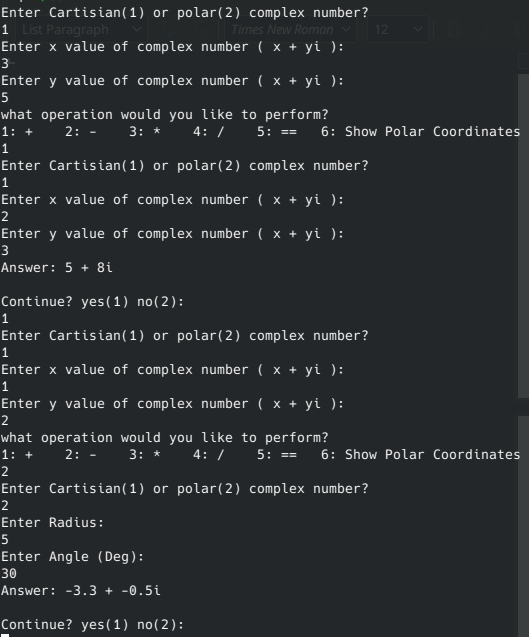
\includegraphics[scale=0.7]{first}
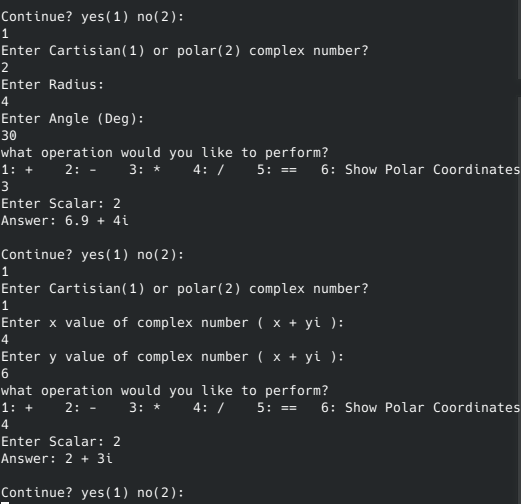
\includegraphics[scale=0.6]{second}
The tester required no change to the original class other than some miscelaneous debugging.

\section{Compilation}
Compiled version included within the base file system. Source folder is included under ./src and can be compiled with mingw g++ or other compilation system. Otherwise the Lab3 folder should be importable to visual studio community. kindly email if any issues with compilation for immediate resolution.

\newpage
\section{Contributions}
\subsection{Chad}
\begin{itemize}
\item Created complex.h
\item Implemented complex.cpp excluding constructors
\item Helped debug test.cpp
\item Created Lab report
\end{itemize}
\subsection{Colton}
\begin{itemize}
\item Created Test.cpp and implemented the tester
\item Figured out conversion between polar and cartaesian
\item Tested class
\end{itemize}

\end{document}